\documentclass[journal]{IEEEtran}

\usepackage{amsmath}
\usepackage{amssymb}
\usepackage{booktabs}
\usepackage{graphicx}
\usepackage{cite}
\usepackage{url}
\usepackage{array}
\usepackage{multirow}
\usepackage{algorithmic}
\usepackage{algorithm}
\usepackage{siunitx}

\graphicspath{{figures/}}

\begin{document}

\title{Supplementary Material:\\Design Equations and Parametric Sizing for Hierarchical Coordination in Large Autonomous Space Swarms}

\author{
  \IEEEauthorblockN{Thijs Hakkenberg}
  \IEEEauthorblockA{Project Dyson, Open Research Initiative\\
  Email: thijs@hakkenberg.com\\
  \url{https://projectdyson.org}}
}

\markboth{IEEE Transactions on Aerospace and Electronic Systems -- Supplementary Material}{}

\maketitle

\begin{abstract}
This document provides supplementary material for ``Design Equations and Parametric Sizing for Hierarchical Coordination in Large Autonomous Space Swarms.'' It contains detailed derivations, extended tables, worked examples, and placeholder sections for NS-3 validation results that accompany the core paper. Section references of the form ``\S X (core)'' refer to the corresponding section of the main paper.
\end{abstract}

\appendix

\renewcommand{\thetable}{S\arabic{table}}
\renewcommand{\thefigure}{S\arabic{figure}}
\setcounter{table}{0}
\setcounter{figure}{0}

%% ===========================================================================
%% SECTION A: FULL NOTATION TABLE
%% ===========================================================================
\section{Full Notation Table}
\label{sec:supp-notation}

This section provides the complete notation reference for all symbols used in the core paper and supplement, extending the compressed notation table in \S I (core). Symbols are organized by functional group.

\begin{table*}[t]
    \centering
    \caption{Complete Notation Reference}
    \label{tab:supp_notation}
    \footnotesize
    \begin{tabular}{@{}llll@{}}
        \toprule
        \textbf{Symbol} & \textbf{Definition} & \textbf{Default} & \textbf{Group} \\
        \midrule
        \multicolumn{4}{@{}l}{\emph{Fleet and Topology}} \\
        $N$ & Fleet size (nodes) & $10^3$--$10^5$ & Fleet \\
        $k_c$ & Cluster size (nodes per coordinator) & 100 & Fleet \\
        $k_r$ & Clusters per regional coordinator & $\lceil N/(k_c \cdot n_r) \rceil$ & Fleet \\
        $n_r$ & Number of regional coordinators & 10 & Fleet \\
        $f_{\text{RF}}$ & Fraction of fleet in RF-backup mode & 0.012 & Fleet \\
        $F$ & Number of orthogonal RF channels & 8 & Fleet \\
        $R$ & Spatial reuse factor & 7 & Fleet \\
        \midrule
        \multicolumn{4}{@{}l}{\emph{Cluster Coordination}} \\
        $T_c$ & Coordination cycle period & 10~s & Cluster \\
        $C_{\text{node}}$ & Per-node bandwidth allocation & 1~kbps & Cluster \\
        $S_{\text{eph}}$ & Status report size & 256~B & Cluster \\
        $S_{\text{cmd}}$ & Command message size & 512~B & Cluster \\
        $C_{\text{coord}}$ & Coordinator ingress link rate (kbps) & --- & Cluster \\
        $C_{\text{coord,info}}$ & Coordinator information-rate requirement & 20.2~kbps & Cluster \\
        $\alpha_{\text{RX}}$ & Ingress fraction of $T_c$ ($= T_{\text{ing}}/T_c$) & 0.908 (30~kbps) & Cluster \\
        $d$ & Campaign duty factor & $[0,1]$ & Cluster \\
        $p_{\text{cmd}}$ & Per-cycle command probability (given ON) & $[0,1]$ & Cluster \\
        $q$ & Unicast fraction of commands & $[0,1]$ & Cluster \\
        $L_{\text{cmd}}$ & Command stagger cycles & 19 (30~kbps) & Cluster \\
        $p_{\text{exc}}$ & Per-node per-cycle reporting probability & 0.10--1.0 & Cluster \\
        $f_{\text{decision}}$ & Raft decisions per cycle & 1 & Cluster \\
        $N_R$ & Raft protocol rounds per decision & 2 & Cluster \\
        \midrule
        \multicolumn{4}{@{}l}{\emph{TDMA Frame}} \\
        $\gamma(R_{\text{PHY}})$ & TDMA slot efficiency & 0.732--0.761 & TDMA \\
        $R_{\text{PHY}}$ & Physical-layer burst rate & 24--50~kbps & TDMA \\
        $R_{\text{FEC}}$ & FEC code rate (LDPC) & 7/8 & TDMA \\
        $O_{\text{frame}}$ & Framing overhead (ASM+addr+ctrl+FCS) & 104~bits & TDMA \\
        $T_{\text{payload}}$ & Information-bit transmission time ($S \times 8 / R_{\text{PHY}}$) & rate-dependent & TDMA \\
        $T_{\text{slot}}$ & Total slot duration & 80--112~ms & TDMA \\
        $T_{\text{guard}}$ & Guard interval (prop+turn+jitter) & 4.7~ms & TDMA \\
        $T_{\text{acq}}$ & Carrier acquisition time (cold-start) & 5~ms & TDMA \\
        \midrule
        \multicolumn{4}{@{}l}{\emph{Channel Model}} \\
        $p_{BG}$, $p_{GB}$ & GE state transition probabilities & 0.50, 0.05 & Channel \\
        $p_G$, $p_B$ & Per-packet loss probability in Good/Bad state & 0.01, 0.90 & Channel \\
        $M_r$ & Maximum retransmission attempts per cycle & 0--2 & Channel \\
        $\pi_G$, $\pi_B$ & GE stationary state probabilities & 0.909, 0.091 & Channel \\
        \midrule
        \multicolumn{4}{@{}l}{\emph{Overhead Metrics}} \\
        $\eta$ & Protocol overhead ($= \eta_0 + d \cdot \eta_{\text{cmd}}$) & 5.6--46\% & Overhead \\
        $\eta_0$ & Architecture-specific overhead & 5.6\% & Overhead \\
        $\eta_{\text{cmd}}$ & Workload-dependent overhead (at $p_{\text{cmd}} = 1$) & 41\% & Overhead \\
        $\eta_{\text{total}}$ & Total utilization ($= \eta + 20.5\%$ baseline) & 26--67\% & Overhead \\
        \bottomrule
    \end{tabular}
\end{table*}


%% ===========================================================================
%% SECTION B: DETAILED GAMMA DECOMPOSITION AND TIMING LEDGER
%% ===========================================================================
\section{Detailed $\gamma$ Decomposition and Timing Ledger}
\label{sec:supp-gamma-timing}

This section provides the full $\gamma$ decomposition and per-slot timing ledger summarized in \S IV-J and \S V-C of the core paper. All $\gamma$ values are computed from the time-domain form (Eq.~3 of the core paper) using unrounded intermediate values.

\subsection{$\gamma$ Decomposition Table}

Table~\ref{tab:supp_gamma_decomposition} decomposes the TDMA slot into its constituent components under CCSDS Proximity-1 framing at 24~kbps PHY rate. The same structure applies at other PHY rates; only the time column rescales (fixed-time overheads $T_{\text{guard}}$ and $T_{\text{acq}}$ remain constant, compressing $\gamma$ at higher rates).

\begin{table}[t]
    \centering
    \caption{$\gamma$ Decomposition from CCSDS Proximity-1 Framing ($S_{\text{eph}} = 256$~B, 24~kbps PHY)}
    \label{tab:supp_gamma_decomposition}
    \footnotesize
    \begin{tabular}{@{}lrrc@{}}
        \toprule
        \textbf{Component} & \textbf{Bits} & \textbf{Time (ms)} & \textbf{Source} \\
        \midrule
        Payload ($S \times 8$) & 2{,}048 & 85.33 & --- \\
        Framing (ASM+addr+ctrl+FCS) & 104 & 4.33 & CCSDS 211.0-B-5 \\
        FEC parity (LDPC 7/8)\textsuperscript{$\ddagger$} & 308 & 12.83 & CCSDS 131.0-B-4 \\
        Guard (prop+turn+jitter) & --- & 4.70 & Prox-1 + geometry \\
        Acquisition (pointing dwell) & --- & 5.00 & Assumed; Prox-1 class \\
        \midrule
        \textbf{Total slot} & \textbf{2{,}460} & \textbf{112.20} & \\
        \textbf{$\gamma_{C,24}$} & \multicolumn{2}{c}{$85.33 / 112.20 = \mathbf{0.761}$} & Eq.~3 (core) \\
        Model~S (no FEC/acq) & \multicolumn{2}{c}{$85.33 / 90.03 = 0.949$} & Eq.~2 (core) \\
        \bottomrule
        \multicolumn{4}{@{}p{0.88\columnwidth}@{}}{\footnotesize \textsuperscript{$\ddagger$}Rate~7/8 LDPC selected to maximize throughput given sufficient ISL link margin ($>$6~dB at 30~kbps); rate-1/2 doubles symbol time, making 30~kbps infeasible. All $\gamma$ values computed from Eq.~3 (core) with unrounded intermediates.}
    \end{tabular}
\end{table}

\subsection{Slot Timing Ledger}

Table~\ref{tab:supp_timing_ledger} is the authoritative timing ledger partitioning every per-slot overhead as either ``in $\gamma$'' (absorbed by the slot efficiency equation) or ``outside $\gamma$'' (separately budgeted in Test~B margin). This ledger is the single reference for all feasibility claims.

\begin{table}[t]
    \centering
    \caption{Slot Timing Ledger: In-$\gamma$ vs.\ Outside-$\gamma$ Components (Model~C, 30~kbps)}
    \label{tab:supp_timing_ledger}
    \footnotesize
    \begin{tabular}{@{}lrrl@{}}
        \toprule
        \textbf{Component} & \textbf{Bits} & \textbf{ms} & \textbf{Scope} \\
        \midrule
        \multicolumn{4}{@{}l}{\emph{In $\gamma$ (per slot)}} \\
        \;\;Payload ($S \times 8$) & 2{,}048 & 68.27 & Data \\
        \;\;Framing (ASM+addr+ctrl+FCS)\textsuperscript{a} & 104 & 3.97 & CCSDS 211.0-B-5 \\
        \;\;FEC parity (LDPC 7/8) & 308 & 10.27 & CCSDS 131.0-B-4 \\
        \;\;Guard (prop+turn+jitter) & --- & 4.70 & Geometry \\
        \;\;Acquisition (cold-start) & --- & 5.00 & Assumed \\
        \midrule
        \multicolumn{4}{@{}l}{\emph{Outside $\gamma$ (per cycle)}} \\
        \;\;ACK mini-slot ($k_c \times 0.5$~ms) & --- & 50 & Conservative \\
        \;\;TX/RX turnaround ($2 \times 2$~ms) & --- & 4 & Half-duplex \\
        \;\;Re-sync preamble (120~bits) & 120 & 4 & Post-turnaround \\
        \;\;Ranging + sync + drift & --- & 19 & CCSDS 414.0-G-2; TCXO \\
        \midrule
        \textbf{In-$\gamma$ subtotal (per slot)} & \textbf{2{,}460} & \textbf{92.2} & $\gamma_{30}\!=\!0.745$ \\
        \textbf{Outside-$\gamma$ subtotal (per cycle)} & --- & \textbf{77} & Test~B margin \\
        \bottomrule
        \multicolumn{4}{@{}p{0.88\columnwidth}@{}}{\footnotesize \textsuperscript{a}Framing bits FEC-encoded per CCSDS practice ($O_{\text{frame}} / (R_{\text{FEC}} R_{\text{PHY}})$). Authoritative $\gamma$ from Eq.~3 (core) with unrounded intermediates.}
    \end{tabular}
\end{table}

\subsection{Measurement Protocol for $\gamma$}

To anchor $\gamma$ in hardware measurements: (a)~measure $T_{\text{acq}}$ (P95) across representative SNR and Doppler conditions; (b)~measure turnaround time and timing jitter to determine $T_{\text{guard}}$; (c)~compute $\gamma$ via Eq.~3 (core); (d)~propagate uncertainty using the closed-form sensitivity: $\partial R_{\text{PHY,min}} / \partial T_{\text{acq}} = (k_c - 1)/(T_c \gamma)$. At nominal parameters this gives $\approx 13.3$~kbps per second of $T_{\text{acq}}$ change.

\subsection{$\gamma$ Consistency Ledger}

The authoritative $\gamma$ values (all from Eq.~3 of the core paper with unrounded intermediates) are: 24~kbps: $T_{\text{slot}}\!=\!112.2$~ms, $\gamma_{24}\!=\!0.761$; 30~kbps: $T_{\text{slot}}\!=\!91.7$~ms, $\gamma_{30}\!=\!0.745$; 35~kbps: $T_{\text{slot}}\!=\!80.0$~ms, $\gamma_{35}\!=\!0.732$; 50~kbps: $T_{\text{slot}}\!=\!59.0$~ms, $\gamma_{50}\!=\!0.695$. All Model~C cold-start ($T_{\text{acq}}\!=\!5$~ms, $T_{\text{guard}}\!=\!4.7$~ms). ACK (0.5~ms per node) is \emph{not} included in $\gamma$; it is separately accounted in Test~B margin. Figs.~4, 6 and Tables~4, 5, 6, 7 of the core paper use these values. Model~S ($\gamma_{24}\!=\!0.949$) appears only in the joint interaction table (illustrative; not for design).


%% ===========================================================================
%% SECTION C: GILBERT-ELLIOTT CHANNEL: FULL MARKOV ANALYSIS
%% ===========================================================================
\section{Gilbert-Elliott Channel: Full Markov Analysis}
\label{sec:supp-ge}

This section provides the complete GE sensitivity analysis and inter-cycle recovery derivation summarized in \S IV-C of the core paper. The GE model is a \emph{what-if design tool}; all results are conditional on unmeasured parameters.

\subsection{Inter-Cycle Recovery Derivation}

Under the GE model with per-cycle state transitions ($p_{GB} = 0.05$, $p_{BG} = 0.50$), each node's ISL experiences independent GE state transitions. The per-cycle recovery probability after $k$ cycles is:
\begin{equation}
    p_{\text{rec}}^{(k)} = \pi_G^{(k)}(1 - p_G^{M_r+1}) + \pi_B^{(k)}(1 - p_B^{M_r+1})
    \label{eq:supp_recovery}
\end{equation}
where $\pi_G^{(k)}$ and $\pi_B^{(k)}$ are the state probabilities at cycle $k$, evolving via the Markov transition matrix:
\begin{equation}
    \begin{bmatrix} \pi_G^{(k+1)} \\ \pi_B^{(k+1)} \end{bmatrix}
    = \begin{bmatrix} 1 - p_{GB} & p_{BG} \\ p_{GB} & 1 - p_{BG} \end{bmatrix}
    \begin{bmatrix} \pi_G^{(k)} \\ \pi_B^{(k)} \end{bmatrix}
\end{equation}
The cumulative recovery CDF is:
\begin{equation}
    F(k) = 1 - \prod_{j=1}^{k}(1 - p_{\text{rec}}^{(j)})
\end{equation}

At default parameters ($p_{BG} = 0.50$, $p_B = 0.90$, $M_r = 2$): mean recovery $= 1.7$ cycles, P95 $= 4$ cycles (DES-verified with 30 MC replications, $N = 10{,}000$).

\subsection{Coherence Regime Discussion}

The GE model transitions once per $T_c$; intra-cycle retransmissions face the same channel state. This makes intra-cycle ARQ structurally ineffective when the coherence time $\tau_c \geq T_c$: under bad-state bursts, all $M_r + 1$ attempts face $p_B = 0.90$, yielding only 27.1\% recovery with $M_r = 2$.

This conclusion is \emph{conditional} on slow fading ($\tau_c \geq T_c$). For fast-fading ($\tau_c \ll T_c$, e.g., rapid tumbling, multipath from reflective surfaces): channel state decorrelates between retransmissions and delivery reaches 98.9\% with $M_r = 2$---intra-cycle ARQ is fully effective.

\textbf{Physical mapping:} $p_{BG} \approx T_c / \bar{T}_B$; default 0.50 is illustrative (no ISL measurements exist). LEO mechanisms include: structural shadowing ($p_{BG} \geq 0.50$), mispointing ($p_{BG} \sim 0.10$), and occultation (${\sim}35$~min; use schedules). Geometric justification: 1~m panel at 2~m separation, $2^\circ$/s tumble rate gives $\tau_c \approx 14$~s $> T_c$; stabilized spacecraft: 50--300~s $\gg T_c$.

\subsection{ARQ Viability Analysis}

ARQ provisioning allocates $M_r$ shared retransmission slots within the superframe margin; the available window is $T_c - T_{\text{ing}} - T_{\text{egr}} - T_{\text{ACK}}$: 680~ms at 30~kbps, 1,830~ms at 35~kbps.

\textbf{Expected demand:} Under GE with $\pi_B = p_{GB}/(p_{BG}+p_{GB}) = 0.091$, $E[\text{failed}] = k_c \pi_B p_B = 100 \times 0.091 \times 0.90 \approx 8.2$ nodes; P95 (binomial, $n\!=\!100$, $p\!=\!0.082$) $\approx 14$ nodes $\times 92$~ms $= 1{,}288$~ms. At 30~kbps: 680~ms $< 1{,}288$ (P95 infeasible); at 35~kbps: 1,830~ms $> 1{,}288$ (P95 feasible).

\textbf{Coherence-regime sensitivity} (what-if; no ISL measurements): (i)~$\tau_c \geq T_c$ \emph{and} $p_B \geq 0.7$: use 35~kbps $+$ inter-cycle recovery (P95~$= 4$ cycles at $p_{BG} = 0.50$); (ii)~$\tau_c \ll T_c$ or $p_B < 0.7$ (benign channel): ARQ effective (98.9\%), 30~kbps suffices. Select $R_{\text{PHY}}$ from Fig.~6(b) of the core paper using measured $\tau_c / T_c$ and $p_B$.

\textbf{$M_r$ selection trade:} $M_r = 0$: no intra-cycle ARQ; accept inter-cycle recovery (AoI penalty $= +T_c$ per lost cycle; P95 $= 4$ cycles); 30~kbps sufficient, full 680~ms margin preserved. $M_r = 1$: recover ${\sim}27\%$ of slow-fading losses intra-cycle; requires 35~kbps (680~ms margin insufficient at 30~kbps). $M_r = 2$: marginally improves recovery to ${\sim}35\%$ under slow fading but consumes ${\sim}184$~ms additional margin; diminishing returns unless $\tau_c \ll T_c$.

\subsection{Sensitivity Sweep}

Fig.~6(b) of the core paper presents the primary sensitivity result: P95 recovery vs.\ $p_{BG}$ for $p_B \in \{0.70, 0.90, 0.95\}$. At $p_{BG} = 0.50$: P95 $= 3$--$5$ cycles; at $p_{BG} = 0.10$ (persistent bad state): 12--18 cycles. Missions should use these design curves with measured $\tau_c$.


%% ===========================================================================
%% SECTION D: DES ARCHITECTURE AND DISTRIBUTIONAL ANALYSIS
%% ===========================================================================
\section{DES Architecture and Distributional Analysis}
\label{sec:supp-des}

This section provides the full distributional analysis and DES architectural details summarized in \S III-A and \S IV-F of the core paper.

\subsection{V\&V Tiers}

The verification and validation hierarchy follows IEEE~1012: \textbf{Tier~1:} DES reproduces analytical means ($<$0.1\% deviation); this confirms implementation correctness, not model validity. Distributional tails (Fig.~\ref{fig:supp_buffer_cdf}) are the DES's incremental contribution beyond closed-form analysis. \textbf{Tier~2:} slot-level simulation reveals ARQ$\times$TDMA coupling; packet-level simulation anchors $\gamma$ (parameter anchoring, not independent validation). \textbf{Tier~3 (absent):} ISL measurements, NS-3 MAC simulation, hardware $\gamma$ measurement (\S\ref{sec:supp-ns3}). No external validation exists.

\subsection{Distributional Tail Analysis}

The DES's sole incremental contribution beyond mean-value agreement is distributional tails under campaign burstiness. Under ON/OFF Markov burst models ($L_{\text{on}} = 100$ cycles), the P99 coordinator ingress shifts ${\sim}25\%$ above the Bernoulli (independent duty-cycle) baseline. A buffer factor $M = 1.30$ at $d = 0.10$ ensures $<$1\% overflow; $M = 1.50$ is required for $d = 0.50$.

\textbf{These are conditional predictions under the Markov ON/OFF assumption, not validated findings.} Under heavy-tailed ON durations (e.g., Pareto-distributed campaign lengths), $M$ would increase; under lighter tails, $M$ would decrease.

\subsection{MMPP/D/1 Corroboration}

Under compound campaign $+$ GE dynamics, the arrival process at the coordinator is well-approximated as MMPP/D/1 (Markov-Modulated Poisson Process with deterministic service). An MMPP/D/1 fluid bound corroborates $M \approx 1.25$--$1.35$ for the assumed parameters. P99 buffer occupancy is ${\sim}20$--$30\%$ above deterministic; closed-form bounds for the exact MMPP/D/1 tail are future work.

\begin{figure}[t]
    \centering
    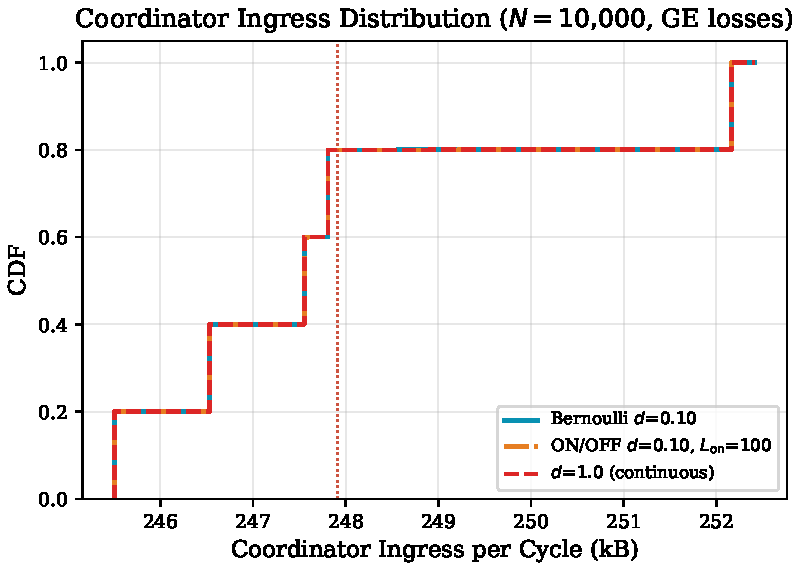
\includegraphics[width=\columnwidth]{fig-coordinator-buffer-cdf.pdf}
    \caption{CDF of per-cycle coordinator ingress bytes ($N = 10{,}000$, $k_c = 100$, GE). Bernoulli $d = 0.10$ (solid): bimodal. ON/OFF $d = 0.10$, $L_{\text{on}} = 100$ (dash-dot): heavier P99. Continuous $d = 1.0$ (dashed): full load. Vertical lines: closed-form means. Buffer factor $M = 1.30$ keeps overflow $< 1\%$ at $d = 0.10$.}
    \label{fig:supp_buffer_cdf}
\end{figure}


%% ===========================================================================
%% SECTION E: THUNDERING HERD AND BEB CONVERGENCE
%% ===========================================================================
\section{Thundering Herd and BEB Convergence}
\label{sec:supp-thundering-herd}

This section provides the full thundering-herd analysis for coordinator election under RF-backup conditions, extending the summary in \S III-B of the core paper.

\subsection{Slotted ALOHA / BEB Analysis}

When a coordinator fails and optical ISL is unavailable, $k_c = 100$ nodes simultaneously attempt Raft election via UHF (2.5~kbps). Under Slotted ALOHA the initial offered load is $G = 25$ (collapse regime; throughput $S = G e^{-G} \approx 0$).

Binary Exponential Backoff (BEB) progressively reduces contention:
\begin{itemize}
    \item Round 0: $W_0 = 4$, $G_0 = 100/4 = 25$ (collapse)
    \item Round 1: $W_1 = 8$, $G_1 = 100/8 = 12.5$ (still overloaded)
    \item Round 2: $W_2 = 16$, $G_2 = 100/16 = 6.25$ (overloaded)
    \item Round 3: $W_3 = 32$, $G_3 = 100/32 = 3.13$ (marginal)
    \item Round 4: $W_4 = 64$, $G_4 = 100/64 = 1.56$ (stable: $S \approx 825$~bps)
\end{itemize}

At $G_4 = 1.56$, throughput $S = G e^{-G} \times R_{\text{UHF}} = 1.56 \times e^{-1.56} \times 2{,}500 \approx 825$~bps. Total election traffic (Raft): $12.8$~KB $= 102{,}400$~bits. Expected election time: $102{,}400 / 825 \approx 124$~s plus BEB convergence overhead, yielding ${\sim}140$--$160$~s total. Raft's randomized timeout (150--300~ms) partially mitigates by staggering candidates.

\subsection{Election--Status Interaction}

During the ${\sim}160$~s RF-backup election, status reporting is \emph{suspended} (hierarchical coordination suspended; see below). Election traffic thus has exclusive use of the 2.5~kbps UHF channel. AoI impact of the suspension: $+$16 missed cycles ($+160$~s), which is modest relative to AoI P99 $= 441$~s.

If status reporting were \emph{not} suspended, the combined load (election 640~bps $+$ 100 beacons $\times$ 51~bps $= 5{,}740$~bps) would exceed UHF capacity (2.5~kbps), causing election failure. Suspension is therefore a \emph{design requirement}, not an optimization.

\subsection{Coordination Suspension Design}

Coordinator ingress ($\geq$27~kbps) exceeds RF-backup capacity (2.5~kbps) by $>$10$\times$; hierarchical coordination is \emph{suspended} during RF-backup operation (beacon-only mode, $\eta \approx 5.7\%$). During suspension, nodes rely on passive safety: conjunction probability per node per 300~s $\approx 10^{-8}$; autonomous collision avoidance is not required during the ${\sim}160$~s election window. TDMA sizing (Sections~IV--V of the core paper) applies to S-band only.

Gaps between elections: $< 1$/yr per cluster (based on 2\%/yr node failure rate applied to coordinators). The compound probability of a coordinator failure occurring during a GE bad-state (triple fault) is $1.8 \times 10^{-5}$/yr, extending election to ${\sim}310$~s.


%% ===========================================================================
%% SECTION F: J2 RE-ASSOCIATION AND DYNAMIC TOPOLOGY
%% ===========================================================================
\section{J2 Re-association and Dynamic Topology}
\label{sec:supp-j2}

This section provides the full dynamic topology analysis under J2 perturbations, extending the summary in \S V-D of the core paper.

\subsection{Walker Constellation Analysis}

J2 analysis (Vallado, \emph{Fundamentals of Astrodynamics}) for a Starlink-like Walker constellation ($53^\circ$ inclination, 550~km altitude, 72~planes $\times$ 22~satellites/plane):

\begin{itemize}
    \item \textbf{Co-orbital re-association:} zero (nodes in the same orbital plane experience identical J2 precession)
    \item \textbf{Cross-plane re-association:} ${\sim}0.014$/orbit fleet-wide (14.8~kB state transfer, $<$0.3\% of per-node budget per cycle)
    \item \textbf{AoI transient:} 33~s per re-association event (3--5~s handoff + state rebuild)
\end{itemize}

Heterogeneous orbits (mixed altitudes or inclinations) produce higher differential precession rates; the re-association frequency scales as $\propto \Delta\Omega / T_c$ where $\Delta\Omega$ is the differential RAAN precession rate between adjacent planes.

\subsection{Worst-Case Boundary Cluster}

At orbital plane interfaces, re-association occurs once per orbit (${\sim}90$~min) as nodes drift between clusters. At 3--5~s optical handoff per event, duty loss $\approx 0.06$--$0.09\%$ of cycle time---negligible for TDMA margin but relevant for coordinator state continuity. Mitigation: overlap zones with dual-cluster membership during handoff; state pre-staging via optical ISL.

\textbf{DES limitation:} static cluster membership is assumed in all DES runs. Dynamic re-association adds $<$0.5\% overhead based on the analytical estimates above; DES verification of dynamic membership is future work.


%% ===========================================================================
%% SECTION G: TOPOLOGY COMPARISON
%% ===========================================================================
\section{Topology Comparison}
\label{sec:supp-topology}

This section provides the extended topology comparison summarized in \S IV-G of the core paper, including the sectorized mesh model and intermediate architecture bounds.

\subsection{Sectorized Mesh Model}

Global-state mesh (full fleet state per node): $O(N^2)$ messages/cycle via gossip; at $N = 10^5$, per-node traffic $\approx 73$~MB/cycle ($\gg 1$~kbps budget). The sectorized mesh reduces this by limiting each node to $k_s = \lceil\sqrt{N}\rceil$ neighbors with a fanout cap of 10: at $N = 10^5$, $k_s = 317$, capped at 10 neighbors. Stress-case overhead: $\eta \approx 65$--$67\%$ with only 3.2\% fleet state coverage.

Both global-state and sectorized mesh are intentional \emph{upper bounds} demonstrating that flat topologies are infeasible at scale under the 1~kbps per-node budget. Hierarchical aggregation achieves $O(k_c)$ per-node cost via coordinator summarization.

\subsection{Centralized Bounds}

Centralized ground processing: $M/D/1$ queue model; $N_{\text{max}} = c \mu_s / r$ ($10^4$ at $c = 1$ server, $10^6$ at $c = 100$). This is an intentional compute bound---propagation latency and uplink spectrum constraints bind first in practice. The centralized model provides a lower bound on protocol overhead (no intra-fleet coordination traffic) but with single-point-of-failure and latency constraints.

Centralized with regional aggregation retains the single-point and latency constraints of pure centralized operation while adding one aggregation layer. This intermediate architecture is not analyzed in detail as it does not change the scaling class ($O(N)$).

\subsection{Partial-State Mesh}

$k$-hop gossip ($O(kN)$ messages/cycle) provides partial fleet state without global guarantees. At $k = 3$: ${\sim}30\%$ of fleet state reachable per node; overhead $\eta \approx 15$--$20\%$ (stress). The partial-state mesh trades coverage completeness for reduced overhead but cannot guarantee coordination consistency (split-brain risk under partitions). The centralized and full-mesh bounds bracket the viable design space; hierarchy occupies the favorable region.


%% ===========================================================================
%% SECTION H: LINK BUDGET DETAIL
%% ===========================================================================
\section{Link Budget Detail}
\label{sec:supp-link-budget}

This section provides the full link budget analysis supporting the PHY rate selection in \S IV-A of the core paper.

\subsection{S-Band ISL Parameters}

S-band 2.2~GHz inter-satellite link budget:
\begin{itemize}
    \item Transmit power: 1~W (+30~dBm)
    \item Antenna gain: 6~dBi patch (both ends)
    \item EIRP: $+36$~dBm
    \item Range: 500~km (intra-cluster nominal)
    \item Free-space path loss: $-151.2$~dB (at 2.2~GHz, 500~km)
    \item System noise temperature: 500~K ($T_{\text{sys}}$; includes antenna, LNA)
    \item $C/N_0 = 64.5$~dB-Hz
    \item At 24~kbps: $E_b/N_0 = 64.5 - 10\log_{10}(24{,}000) = 20.7$~dB; margin $= 20.7 - 4.8 = 15.9$~dB (LDPC 7/8 threshold)
    \item At 35~kbps: $E_b/N_0 = 64.5 - 10\log_{10}(35{,}000) = 19.1$~dB; margin $= 19.1 - 4.8 = 14.3$~dB
    \item Aggregate capacity: $>$200~kbps at 6~dB margin threshold
    \item Per-node allocation: 1~kbps at $k_c = 100$ with ${\sim}50\%$ margin
\end{itemize}

\subsection{UHF RF-Backup Parameters}

UHF omnidirectional backup link:
\begin{itemize}
    \item Frequency: 400~MHz band
    \item Transmit power: 0.5~W (+27~dBm)
    \item Antenna gain: 0~dBi (omnidirectional)
    \item $E_b/N_0 = 16.5$~dB at 1~kbps
    \item Maximum sustainable rate: ${\sim}2.5$~kbps
    \item Purpose: safe-mode beacons and coordinator election only
\end{itemize}

RF backup is necessary because tumbling spacecraft cannot maintain optical pointing. The hierarchy is suspended during RF-backup operation (\S\ref{sec:supp-thundering-herd}).

\subsection{Sensitivity Analysis}

$\pm 3$~dB link margin variation maps to per-node budget $\in [0.5, 2]$~kbps:
\begin{itemize}
    \item At 0.5~kbps ($-3$~dB): stress-case $\eta_{\text{total}} \approx 92\%$ (infeasible; TDMA margin negative)
    \item At 1~kbps (nominal): $\eta_{\text{total}} \approx 67\%$ (feasible; TDMA margin 680~ms at 30~kbps)
    \item At 2~kbps ($+3$~dB): $\eta_{\text{total}} \approx 33\%$ (comfortable; TDMA non-binding)
\end{itemize}

At $\geq$2~kbps, stress-case $\eta$ halves to ${\sim}23\%$ and TDMA sizing becomes non-binding; only Test~A (byte budget) is required.


%% ===========================================================================
%% SECTION I: GAMMA-CONDITIONAL PHY RATE LOOKUP
%% ===========================================================================
\section{$\gamma$-Conditional PHY Rate Lookup}
\label{sec:supp-gamma-lookup}

This section provides the full $\gamma$-conditional lookup table and acquisition mode sensitivity analysis from \S IV-J of the core paper, intended as a practitioner reference.

\begin{table}[t]
    \centering
    \caption{$\gamma$-Conditional PHY Rate Lookup ($k_c = 100$, $S = 256$~B, $T_c = 10$~s)}
    \label{tab:supp_gamma_phy_lookup}
    \footnotesize
    \begin{tabular}{@{}cccc@{}}
        \toprule
        \textbf{Measured $\gamma$} & $R_{\text{PHY,min}}$ & \textbf{Margin} & \textbf{Application Note} \\
        \midrule
        $[0.50, 0.65)$ & $\geq$50~kbps & $>$40\% & Conservative; high-overhead modem \\
        $[0.65, 0.70)$ & 40~kbps & 20--25\% & Includes ARQ margin \\
        $[0.70, 0.80)$ & \textbf{35~kbps} & \textbf{12--19\%} & \textbf{Recommended (CCSDS default)} \\
        $[0.80, 0.90)$ & 30~kbps & 7--15\% & Minimum; no ARQ margin \\
        $[0.90, 1.00)$ & 25~kbps & 5--10\% & Ideal modem (continuous tracking) \\
        \bottomrule
        \multicolumn{4}{@{}p{0.88\columnwidth}@{}}{\footnotesize Margin $= (T_c - T_{\text{ing}} - T_{\text{egr}} - T_{\text{ACK}})/T_c$ (Table~\ref{tab:supp_timing_ledger}). Practitioners: measure $\gamma$ per the protocol in \S\ref{sec:supp-gamma-timing}, then select $R_{\text{PHY}}$ from this table. For $k_c \neq 100$ or $S \neq 256$~B: recompute via Algorithm~1 (core).}
    \end{tabular}
\end{table}

\subsection{Full Consistency Ledger}

The $\gamma$ consistency ledger ensures all tables, figures, and equations in both the core paper and supplement use identical values:

\begin{table}[t]
    \centering
    \caption{$\gamma$ Consistency Ledger (Model~C, Cold-Start)}
    \label{tab:supp_consistency}
    \footnotesize
    \begin{tabular}{@{}ccccc@{}}
        \toprule
        $R_{\text{PHY}}$ (kbps) & $T_{\text{payload}}$ (ms) & $T_{\text{slot}}$ (ms) & $\gamma$ & Feasibility \\
        \midrule
        24 & 85.33 & 112.2 & 0.761 & Infeasible ($-$1,300~ms) \\
        30 & 68.27 & 91.7 & 0.745 & Min.\ viable (680~ms) \\
        \textbf{35} & \textbf{58.51} & \textbf{80.0} & \textbf{0.732} & \textbf{Recommended (1,830~ms)} \\
        50 & 40.96 & 59.0 & 0.695 & Ample ($>$4,000~ms) \\
        \bottomrule
    \end{tabular}
\end{table}

\subsection{Acquisition Mode Sensitivity}

Three acquisition modes are evaluated: \emph{cold-start} ($T_{\text{acq}}\!=\!5$~ms, conservative, CCSDS Prox-1 default), \emph{reacquire} ($T_{\text{acq}}\!=\!2$~ms, carrier relock after brief interruption), \emph{tracking} ($T_{\text{acq}}\!=\!0$, continuous carrier lock).

At cold-start (including ACK): 30~kbps margin $= 680$~ms (6.8\% of $T_c$); 35~kbps margin $= 1{,}830$~ms (18.3\%); 24~kbps deficit $= -1{,}300$~ms (infeasible). At reacquire: 30~kbps margin $= 1{,}068$~ms (10.7\%).

\textbf{Breaking points:} 35~kbps remains feasible up to $T_{\text{acq}} \approx 19$~ms; 30~kbps up to $T_{\text{acq}} \approx 7.4$~ms. \textbf{Slow-acquisition hardware} ($T_{\text{acq}} > 10$~ms, common in low-cost CubeSat radios): recommend $R_{\text{PHY}} \geq 40$~kbps (per Fig.~4 of the core paper). The 35~kbps cold-start recommendation is appropriate for CCSDS-class hardware.


%% ===========================================================================
%% SECTION J: CLAIM MAP BY EVIDENCE TIER
%% ===========================================================================
\section{Claim Map by Evidence Tier}
\label{sec:supp-claim-map}

This section provides the full claim-to-evidence mapping from \S V-A of the core paper, extended with an NS-3 column for future validation results.

\begin{table*}[t]
    \centering
    \caption{Claim Map by Evidence Tier (Extended with NS-3 Column)}
    \label{tab:supp_claim_map}
    \footnotesize
    \begin{tabular}{@{}lccccccc@{}}
        \toprule
         & \multicolumn{3}{c}{\textbf{Tier~1 (Internal)}} & \textbf{Tier~2} & \textbf{Std.-based param.} & \textbf{Tier~3} & \textbf{NS-3} \\
        \cmidrule(lr){2-4} \cmidrule(lr){5-5} \cmidrule(lr){6-6} \cmidrule(lr){7-7} \cmidrule(lr){8-8}
        \textbf{Result} & \textbf{Analyt.} & \textbf{DES} & \textbf{Distrib.} & \textbf{Slot-sim} & \textbf{CCSDS $\gamma$}\textsuperscript{$\ddagger$} & \textbf{Ext.} & \textbf{Sim.}\textsuperscript{$\S$} \\
        \midrule
        $\eta_0 \approx 5.6\%$ & \S IV-E & $<$0.1\% & --- & --- & --- & --- & --- \\
        $\eta_S \approx 46\%$ & \S IV-E & $<$0.1\% & CDF & --- & --- & --- & --- \\
        Coord.\ 24--30~kbps & Eq.~6 & --- & CDF & Exact & 24 infeas. & --- & --- \\
        Margin 680~ms\textsuperscript{$\dagger$} & Tbl.~4 & --- & --- & Exact & --- & --- & --- \\
        $\gamma$ sensitivity & Tbl.~S5 & --- & --- & Conf. & $\gamma\!=\!0.76$ & --- & --- \\
        ARQ infeas.\ (GE) & Markov & --- & --- & 52.7\% & Conf. & --- & --- \\
        35~kbps recommended & Tbl.~S5 & --- & --- & ARQ & $\gamma_{35}\!=\!0.732$ & --- & --- \\
        1~kbps per-node budget & --- & --- & --- & --- & Link budget & --- & --- \\
        AoI P99 $= 440$~s & Eq.~5 & Conf. & --- & --- & --- & --- & --- \\
        GE P95 rec.\ 4 cyc. & Markov & Conf. & CDF & --- & --- & --- & --- \\
        $L_{\text{cmd}}(q)$ stagger & Eq.~8 & --- & --- & Conf. & --- & --- & --- \\
        TDMA decoupling & --- & --- & --- & ($M_r\!=\!0$) & --- & --- & --- \\
        ARQ coupling & --- & --- & --- & ($M_r\!\geq\!1$) & --- & --- & --- \\
        $T_c^{\text{fleet}}$ reuse ($R\!=\!7$) & Eq.~4 & --- & --- & --- & --- & NS-3 & --- \\
        Antenna sched. & --- & --- & --- & --- & --- & Future & --- \\
        MAC contention & --- & --- & --- & --- & --- & Future & --- \\
        \bottomrule
        \multicolumn{8}{@{}p{0.92\textwidth}@{}}{\footnotesize\textsuperscript{$\dagger$}30~kbps Model~C (Table~4 of core). Model~S at 24~kbps: 611~ms. \textsuperscript{$\ddagger$}Packet-level $\gamma$ is a \emph{standards-based parameter estimate} (\S IV-J of core), not independent validation. \textsuperscript{$\S$}NS-3 column: placeholder for future validation runs (\S\ref{sec:supp-ns3}).}
    \end{tabular}
\end{table*}


%% ===========================================================================
%% SECTION K: NS-3 VALIDATION: FULL METHODOLOGY
%% ===========================================================================
\section{NS-3 Validation: Full Methodology}
\label{sec:supp-ns3}

This section describes the planned NS-3 validation methodology for the analytical and DES results presented in the core paper. Results will be populated after NS-3 simulation runs complete.

% TODO: Populate after NS-3 runs complete

\subsection{Simulation Setup}
The NS-3 scenario implements a star-topology TDMA cluster using NS-3 3.41+
core networking primitives (\texttt{PointToPointNetDevice},
\texttt{BurstErrorModel}, \texttt{FlowMonitor}). No code or equations
are shared with the Python analytical model or DES.

\textbf{Key differences from the analytical model:}
\begin{itemize}
    \item Framing: 88 bits (ASM+addr+ctrl+FCS) vs.\ 104 bits in Model~C
    \item Acquisition: stochastic LogNormal($\mu = \ln 5$\,ms, $\sigma = 0.3$) vs.\ fixed 5\,ms
    \item Channel: NS-3 \texttt{BurstErrorModel} vs.\ our custom GE implementation
    \item Scheduling: NS-3 event-driven packet handling vs.\ time-slot aggregation
\end{itemize}

\subsection{Parameter Sweeps}
PHY rate: $\{20, 24, 28, 30, 32, 35, 40, 50\}$~kbps.
Cluster size: $\{50, 100, 200, 500\}$.
GE states: no-loss, default ($p_{BG} = 0.50$, $p_B = 0.90$), severe.
ARQ: $M_r \in \{0, 1, 2\}$.

\subsection{Results}
[Placeholder: full sweep results tables and additional figures.]


%% ===========================================================================
%% SECTION L: ALTERNATIVE TDMA DESIGNS: EXTENDED ANALYSIS
%% ===========================================================================
\section{Alternative TDMA Designs: Extended Analysis}
\label{sec:supp-alternatives}

This section analyzes four alternative TDMA slot structures beyond the cold-start baseline used in the core paper. Detailed NS-3 comparison results will be added when available.

% TODO: Populate with detailed NS-3 comparison

Four slot structures are analyzed:

\textbf{Config A (Cold-start, baseline):} Single-packet per slot with full
carrier acquisition. This is the conservative assumption used throughout the
core paper.

\textbf{Config B (Multi-packet burst):} Three packets per slot with a single
acquisition phase. Inter-packet gap: 0.5\,ms. Amortizes acquisition overhead
across 3 payloads.

\textbf{Config C (Tracking mode):} First slot uses cold-start acquisition;
subsequent slots maintain carrier tracking ($T_{\mathrm{acq}} = 0$).
Models continuous-carrier receivers.

\textbf{Config D (Bitmap ACK):} Same data slots as Config~A, but coordinator
sends a 13-byte aggregate bitmap ACK instead of individual 0.5\,ms ACK
mini-slots. Frees coordinator egress time.

[Placeholder: detailed analytical derivations and NS-3 sweep results for each config.]


%% ===========================================================================
%% SECTION M: SIZING WALKTHROUGH WORKED EXAMPLE
%% ===========================================================================
\section{Sizing Walkthrough Worked Example}
\label{sec:supp-walkthrough}

This section provides the complete sizing walkthrough referenced in \S V-C of the core paper, with step-by-step annotations mapping each computation to Algorithm~1 (core).

\subsection{Problem Statement}

Size a hierarchical coordination cluster with parameters: $k_c = 100$ nodes, campaign duty factor $d = 0.10$, candidate PHY rate 35~kbps. Determine feasibility under both Test~A and Test~B with $M_r = 1$ intra-cycle retransmission.

\subsection{Step 1: Compute $\gamma$ (Algorithm~1, Line~1)}

From the slot efficiency equation (Eq.~3 of the core paper):
\begin{align*}
    T_{\text{payload}} &= \frac{256 \times 8}{35{,}000} = 58.51~\text{ms} \\
    T_{\text{FEC}} &= \frac{256 \times 8 \times (1/0.875 - 1)}{35{,}000} = 8.36~\text{ms} \\
    T_{\text{framing}} &= \frac{104}{0.875 \times 35{,}000} = 3.39~\text{ms} \\
    T_{\text{slot}} &= 58.51 + 8.36 + 3.39 + 4.70 + 5.00 = 79.97~\text{ms} \\
    \gamma_{35} &= 58.51 / 79.97 = 0.732
\end{align*}

\textbf{Annotation:} The FEC rate 7/8 expands payload by $1/R_{\text{FEC}} - 1 = 1/7$; framing bits (104) are also FEC-encoded per CCSDS practice. Guard (4.70~ms) and acquisition (5.00~ms) are fixed-time overheads independent of PHY rate.

\subsection{Step 2: Test A --- Byte Budget (Algorithm~1, Line~3)}

\begin{align*}
    \eta_0 &= 5.6\% \quad \text{(heartbeats 5.1\% + summaries 0.4\% + elections 0.1\%)} \\
    \eta_{\text{cmd}} &= d \times p_{\text{cmd}} \times \frac{S_{\text{cmd}} \times 8}{C_{\text{node}} \times T_c} \\
                      &= 0.10 \times 1.0 \times \frac{512 \times 8}{1{,}000 \times 10} = 4.1\% \\
    \eta_{\text{total}} &= \eta_0 + \eta_{\text{cmd}} + \eta_{\text{baseline}} \\
                        &= 5.6\% + 4.1\% + 20.5\% = 30.2\% \quad \checkmark~(< 100\%)
\end{align*}

\textbf{Annotation:} The 20.5\% baseline is the periodic ephemeris status report (256~B/cycle $= 204.8$~bps at 1~kbps), always present and topology-invariant. $\eta_{\text{cmd}}$ uses $p_{\text{cmd}} = 1.0$ (command every active cycle) with $d = 0.10$ (10\% of cycles active).

\subsection{Step 3: Test B --- TDMA Airtime (Algorithm~1, Lines~4--6)}

\begin{align*}
    T_{\text{ing}} &= (k_c - 1) \times T_{\text{slot}} = 99 \times 80.0 = 7{,}920~\text{ms} \\
    T_{\text{egr}} &= T_{\text{cmd}} + T_{\text{hb}} + T_{\text{sync}} + T_{\text{turn}} \\
                   &= 160 + 24 + 4 + 4 = 192~\text{ms} \\
    T_{\text{ACK}} &= k_c \times 0.5 = 50~\text{ms} \\
    \text{margin} &= T_c - T_{\text{ing}} - T_{\text{egr}} - T_{\text{ACK}} \\
                  &= 10{,}000 - 7{,}920 - 192 - 50 = 1{,}838~\text{ms} \quad \checkmark
\end{align*}

\textbf{Annotation:} Ingress is the dominant term (79.2\% of $T_c$). Egress includes FEC-encoded command broadcast (512~B at 35~kbps with LDPC 7/8), heartbeat (64~B), re-sync preamble (120~bits), and two TX/RX turnarounds ($2 \times 2$~ms). The 1,838~ms margin (18.4\% of $T_c$) is the design target for accommodating ARQ and unmodeled overheads.

\subsection{Step 4: ARQ Feasibility (Algorithm~1, Line~11)}

With $M_r = 1$ retransmission slot: $T_{\text{ARQ}} = 1 \times 80.0 = 80$~ms.

Residual margin: $1{,}838 - 80 = 1{,}758$~ms $> 0$ \checkmark.

Under GE losses: P95 demand $= 14$ failed nodes $\times 80$~ms $= 1{,}120$~ms $< 1{,}758$~ms \checkmark.

\textbf{Annotation:} The ARQ demand is well within margin at 35~kbps. Compare with 30~kbps where margin is only 680~ms and P95 demand (1,288~ms) exceeds it---confirming the 35~kbps recommendation.

\subsection{Step 5: Heuristic Cross-Check}

The design heuristic provides a lower-bound verification:
\begin{align*}
    \alpha_{\text{RX}} &= T_{\text{ing}} / T_c = 7{,}920 / 10{,}000 = 0.792 \\
    R_{\text{PHY,min}} &= \frac{C_{\text{coord,info}}}{\gamma \times \alpha_{\text{RX}}} = \frac{20.2}{0.732 \times 0.792} = 34.8~\text{kbps}
\end{align*}

Since $34.8 < 35$~kbps \checkmark. The heuristic underestimates because it ignores egress time; it equals Test~B exactly when $M_r = 0$ and egress $= 0$.

\subsection{Summary}

\begin{table}[t]
    \centering
    \caption{Sizing Walkthrough Summary ($k_c = 100$, $d = 0.10$, 35~kbps)}
    \label{tab:supp_walkthrough}
    \footnotesize
    \begin{tabular}{@{}llcc@{}}
        \toprule
        \textbf{Step} & \textbf{Test} & \textbf{Result} & \textbf{Status} \\
        \midrule
        1 & $\gamma_{35}$ & 0.732 & --- \\
        2 & Test~A ($\eta_{\text{total}}$) & 30.2\% & \checkmark \\
        3 & Test~B (margin) & 1,838~ms & \checkmark \\
        4 & ARQ ($M_r = 1$) & 1,758~ms residual & \checkmark \\
        5 & Heuristic & 34.8~kbps $< 35$ & \checkmark \\
        \bottomrule
    \end{tabular}
\end{table}

All tests pass with comfortable margin. The 35~kbps PHY rate at $k_c = 100$ with $d = 0.10$ provides 18.4\% superframe margin, accommodates $M_r = 1$ ARQ under GE losses (P95), and maintains Test~A utilization at 30.2\%. For other parameter combinations, substitute deployment-specific values into Algorithm~1 (core) or use the $\gamma$-conditional lookup in Table~\ref{tab:supp_gamma_phy_lookup}.

\end{document}
